\section{Electron energy loss spectroscopy}
\label{sec:eels}

A powerful technique to explore the local electronic properties
of nanoscale materials is electron energy loss spectroscopy (EELS)
within the transmission electron microscope (TEM).
%
As illustrated in the left panel of Fig.~\ref{fig:EELS},
in this technique a magnetic
prism is used to deflect the TEM
electron beam that has just crossed the sample
and then the distribution of energy losses $\Delta E$ can be recorded.
%
This distributions provides important information on various
aspects of the sample.

The EELS spectra are divided into three main regions.
%
The first one is the zero-loss region, centered at $\Delta E=0$
and that contains the contribution of both elastic scatterings
as well as that of those electrons that have not interacted with the
sample.
%
This region is characterised by a strong, narrow peak called
the Zero Loss Peak (ZLP), which is larger than the contribution
from inelastic scattering by several orders of magnitude.
%
The second region is the low-loss region, for energy losses
$\Delta E \lsim 50$ eV which contains information
on features such as plasmons, excitons, phonons, and
intra-band transitions.
%
Finally for $\Delta E \gsim 50$ eV one has the core-loss region,
which is used to provide compositional information
on the sample.
%
The right panel of Fig.~\ref{fig:EELS} displays
a representative EELS spectrum taken on a WS$_2$ nanostructure,
focusing on the low-loss region.
%
 The inset displays the zero loss peak, to illustrate that
 its magnitude is larger than the signal by several
 orders of magnitude.
 
%%%%%%%%%%%%%%%%%%%%%%%%%%%%%%%%%%%%%%%%%%%%%%%
\begin{figure}[H]
    \centering
    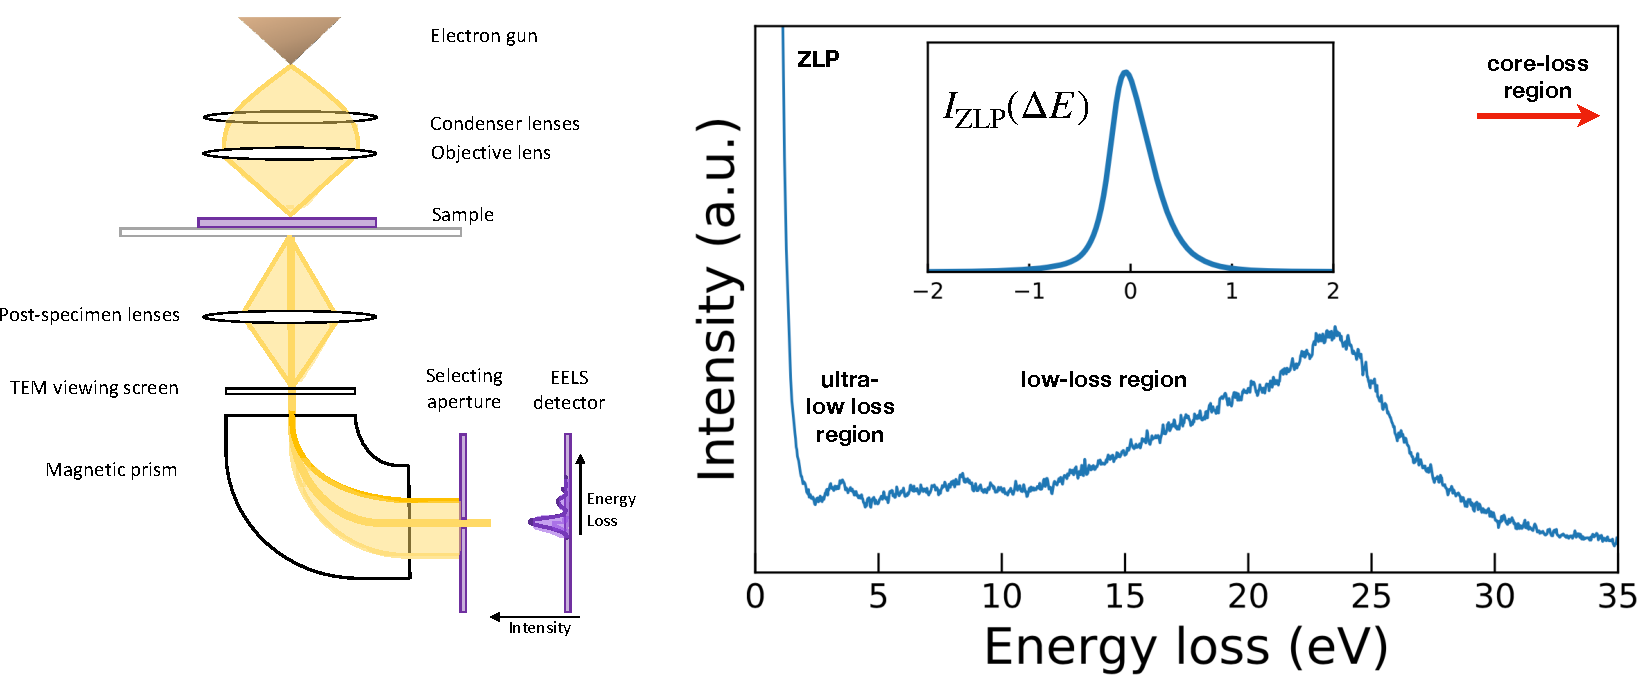
\includegraphics[width=0.9\textwidth]{plots/EELS.pdf}
    \caption{Left: in electron energy loss spectroscopy, a magnetic
      prism is used to deflect the electron beam that has crossed the sample
      and then the distribution of energy losses can be recorded.
      Right: example of a typical EELS spectrum for the low-loss
      region.
      %
      The inset displays the zero loss peak, to illustrate that
      its magnitude is larger than the signal by several
      orders of magnitude.
      }
    \label{fig:EELS}
\end{figure}
%%%%%%%%%%%%%%%%%%%%%%%%%%%%%%%%%%%%%%%%%%%%%%%%5
